\chapter{Methodology}

\section{Research approach}

This project used a quantitative secondary-data approach combined with
software-system evaluation. The investigation examined whether a small
project-specific head could learn outfit compatibility from published fashion data and whether
its scores could support a practical recommendation application. The research
therefore covered both model performance and the behaviour of the complete
recommendation process.

The project did not conduct interviews, questionnaires or other participant
research. The available evidence is limited to offline model evaluation,
controlled comparisons and functional system testing.

The complete technical route is shown in Figure~\ref{fig:technical-route}.
It separates secondary-data preparation and frozen feature extraction from
compatibility learning, controlled evaluation and application deployment.

\begin{figure}[htbp]
  \centering
  \resizebox{\textwidth}{!}{%
  \begin{tikzpicture}[
    font=\small,
    data/.style={draw=wmgdarkblue!55, rounded corners=2pt, align=center,
      minimum width=31mm, minimum height=11mm, fill=gray!7},
    process/.style={data, fill=wmgblue!11, draw=wmgblue!70},
    artefact/.style={data, fill=green!7, draw=green!45!black},
    arrow/.style={-{Latex[length=2.2mm]}, thick, draw=wmgdarkblue!70}
  ]
    \node[data] (polyvore) {Polyvore disjoint\\images and metadata};
    \node[process, right=7mm of polyvore] (mapping) {Four-position mapping\\and negative construction};
    \node[process, right=7mm of mapping] (siglip) {Frozen SigLIP\\feature extraction};
    \node[artefact, right=7mm of siglip] (tensors) {Processed embeddings\\and outfit tensors};

    \node[process, below=13mm of mapping] (training) {Compatibility-head\\training};
    \node[process, right=7mm of training] (selection) {Validation selection\\and calibration};
    \node[artefact, right=7mm of selection] (checkpoint) {Selected checkpoint\\and abstract prototypes};

    \node[process, below=13mm of training] (evaluation) {Baselines, FITB, ablation,\\bias and generalisation tests};
    \node[process, right=7mm of evaluation] (runtime) {Constraint filtering and\\exact candidate search};
    \node[artefact, right=7mm of runtime] (prototype) {Cove recommendation\\prototype};

    \draw[arrow] (polyvore) -- (mapping);
    \draw[arrow] (mapping) -- (siglip);
    \draw[arrow] (siglip) -- (tensors);
    \draw[arrow] (tensors.south) -- ++(0,-5mm) -| (training.north);
    \draw[arrow] (training) -- (selection);
    \draw[arrow] (selection) -- (checkpoint);
    \draw[arrow] (checkpoint.south) -- ++(0,-5mm) -| (runtime.north);
    \draw[arrow] (training) -- (evaluation);
    \draw[arrow] (evaluation) -- (runtime);
    \draw[arrow] (runtime) -- (prototype);
  \end{tikzpicture}}
  \caption{Technical route from secondary fashion data to the evaluated prototype}
  \label{fig:technical-route}
\end{figure}


\section{Data and ethical scope}

The main model was trained and evaluated using files distributed as the
Polyvore Outfits disjoint benchmark described by
\textcite{vasileva2018typeaware} and linked from the authors' repository
\parencite{vasileva2018repository}. The local copy was obtained on 21 August
2026. The three metadata files contain 16,995 training, 3,000 validation and
15,145 test outfits. Their outfit identifiers do not overlap. A reproducible
local audit nevertheless found non-zero item-identifier overlap: 3,781 between
training and validation, 84 between training and test, and 34 between
validation and test. The dissertation therefore uses \emph{disjoint} as the
published split name and does not claim that the local artefact establishes
strict product-level separation. This residual overlap is considered in the
validity analysis.

The application supports four clothing positions: an inner top, an optional
outer layer, a bottom and shoes. The published compatibility files contained
33,990 training, 6,000 validation and 30,290 test rows. Processing retained
rows with at least three distinct supported positions and available
embeddings, yielding 18,243 training, 3,274 validation and 16,062 test
examples. The retained label counts were 9,121 positive and 9,122 negative
training examples, 1,637 of each label for validation, and 8,031 of each label
for test. The corresponding exclusions for insufficient supported positions
were 15,747, 2,726 and 14,228 rows; 1,348, 220 and 1,414 of these rows also
contained a duplicate supported position. No retained row lacked an embedding.
Positive and same-type corrupted negative rows were read from the published
compatibility file for their own split; negatives were not generated by
drawing items across split boundaries.

Polyvore was used to learn compatibility relationships. The separately
obtained \emph{Zara Products} dataset was downloaded from its Kaggle record on
11 August 2026 \parencite{parrenolara2024zara}. It was not added to the
compatibility labels and was used only for garment-recognition preparation and
feature-domain diagnostics.
User-uploaded photographs remain on the local device and were not used as
research data.

\section{Recommendation-model development}

SigLIP was used to convert each garment image into a numerical visual
representation \parencite{zhai2023siglip}. The implementation used
\texttt{google/siglip-base-patch16-224}; the local Hugging Face cache resolved
\texttt{main} to revision
\texttt{7fd15f0689c79d79e38b}\allowbreak\texttt{1c2e2e2370a7bf2761ed}
\parencite{google2024siglipmodelcard}. SigLIP itself was not retrained. Feature
extraction ran without gradient updates, and the resulting 768-dimensional
item vectors were cached before head training. The optimiser received only the
project-specific head parameters, so encoder weights were never included in
an update step. This substantially reduced the
amount of computation required and allowed every comparison model to use the
same visual information.

A small neural model was then trained to assign one compatibility score to a
complete outfit. The model combines two forms of information: an overall
summary of the garments and the visual differences between garment pairs.
Clothing-position information is also supplied so that, for example, the
relationship between a top and shoes can be distinguished from the relationship
between two other positions.

The compatibility head contains 379,265 trainable parameters. A 768-dimensional
input is layer-normalised and projected to 256 dimensions with a linear layer
and GELU. A learned 32-dimensional embedding for each of four clothing
positions is concatenated to the projected item. The model forms a masked mean
of the present items and a second masked mean of the six absolute pairwise
difference vectors. Their concatenation is passed through a
$576\rightarrow256\rightarrow128\rightarrow1$ multilayer perceptron, with
GELU activations and dropout of 0.20 before the second linear layer. It was
trained to distinguish positive outfits from constructed negative outfits.
Its output is later used to rank recommendations. The training objective itself
is compatibility classification rather than direct user-preference prediction.

Figure~\ref{fig:model-architecture} shows the implemented compatibility head.
The trainable component receives frozen item embeddings and a position mask,
then combines a masked outfit summary with explicit pairwise differences before
producing one compatibility logit.

\begin{figure}[htbp]
  \centering
  \resizebox{0.96\textwidth}{!}{%
  \begin{tikzpicture}[
    font=\small,
    box/.style={draw=wmgdarkblue!55, rounded corners=2pt, align=center,
      text width=34mm, minimum height=11mm, fill=wmgblue!6},
    key/.style={box, fill=wmgblue!14, draw=wmgblue!75},
    score/.style={box, fill=green!8, draw=green!45!black},
    arrow/.style={-{Latex[length=2.2mm]}, thick, draw=wmgdarkblue!70}
  ]
    \node[box] (input) at (0,3.2) {Four 768-dimensional\\SigLIP item embeddings\\plus position mask};
    \node[key] (projection) at (4.6,3.2) {Layer normalisation,\\linear projection and GELU};
    \node[key] (slots) at (9.2,3.2) {Concatenate learned\\position embeddings};

    \node[box] (pooled) at (6.9,1.2) {Masked mean\\outfit summary};
    \node[box] (pairs) at (11.5,1.2) {Six absolute pairwise\\difference vectors\\and masked mean};
    \node[key] (concat) at (9.2,-0.9) {Concatenate global and\\pairwise summaries};
    \node[key] (mlp) at (13.8,-0.9) {Two-layer MLP\\with GELU and dropout};
    \node[score] (logit) at (18.4,-0.9) {Compatibility logit\\and calibrated score};

    \draw[arrow] (input) -- (projection);
    \draw[arrow] (projection) -- (slots);
    \draw[arrow] (slots) -- (pairs);
    \draw[arrow] (slots) -- (pooled);
    \draw[arrow] (pairs) -- (concat);
    \draw[arrow] (pooled) -- (concat);
    \draw[arrow] (concat) -- (mlp);
    \draw[arrow] (mlp) -- (logit);
  \end{tikzpicture}}
  \caption{Architecture of the task-specific lightweight compatibility model}
  \label{fig:model-architecture}
\end{figure}


Training was limited to 12 epochs and used validation performance to select the
saved checkpoint. Three predefined random seeds were used to examine whether
results depended heavily on one training run. The test set was kept separate
from model selection.

The processed labels were already balanced, so the final model did not apply
additional positive-class weighting. Alternative weighting by outfit length
was tested but did not satisfy the complete acceptance criteria. The unweighted
model was therefore retained. Detailed settings and the rejected weighting
experiment are reserved for the appendices.

\section{Comparative experiments}

The proposed model was first compared with random ranking and a non-learned
SigLIP similarity baseline. These controls test whether the model performs
above chance and whether learning garment relationships adds value beyond the
frozen visual representation.

Three further models represented established directions in outfit-recommendation
research: a bidirectional LSTM based on \textcite{han2017bilstm}, a type-aware
pairwise model based on \textcite{vasileva2018typeaware}, and a
Transformer-based set model informed by \textcite{sarkar2023outfittransformer}.
They used the same processed data, frozen image representations and training
conditions as the proposed model. They are controlled implementations of the
main architectural ideas rather than exact reproductions of the published
systems.

Two ablation experiments were also conducted. One removed clothing-position
information, and the other removed the module that explicitly compares garment
pairs. The purpose was to determine whether these components made a measurable
contribution when the rest of the experimental conditions remained unchanged.

\section{Model and system evaluation}

Compatibility classification was evaluated using several complementary
measures. ROC--AUC measured how reliably positive outfits received higher
scores than negative outfits \parencite{fawcett2006roc}. Accuracy, balanced
accuracy, precision, recall, F1 and the confusion matrix were used to examine
classification behaviour at the selected threshold. Calibration measures were
reported separately because a model can rank examples correctly while still
producing overconfident scores \parencite{guo2017calibration}.

Recommendation performance was examined through the official fill-in-the-blank
task. One garment is removed from an outfit and the model must select the
correct replacement from four candidates. The correct answer was matched
through the outfit identifier because the answers in the disjoint data are
shuffled. Only questions compatible with the project's four clothing positions
were retained, and the retained proportion is reported with the result.

Confidence intervals were estimated by percentile bootstrap resampling
\parencite{efron1994bootstrap}. The selected-model AUC interval used 1,000
resamples of the 16,062 test rows; the selected FITB interval used 2,000
resamples of 4,468 retained questions. Structural-ablation intervals used
5,000 paired resamples of those questions after averaging correctness over the
three seeds. The exact-versus-quota score-loss interval used 2,000 resamples of
the 18 query-level differences. All reported intervals use the 2.5th and
97.5th percentiles. The same questions and random seeds
were used when comparing the complete model with an ablation, allowing their
differences to be assessed directly. Training, validation and test behaviour
were also compared to identify evidence of overfitting.

Expected calibration error used ten equal-width probability bins on the
validation examples. Scalar temperature scaling minimised validation binary
cross-entropy and did not use the test labels. Empty bins contributed no error;
each populated bin was weighted by its share of validation examples.

The complete application was tested separately from the classifier. Candidate
availability was checked under different weather and style conditions. Search
experiments examined whether the previous quota-based method could miss
higher-scoring combinations and measured the time required to search the
complete filtered candidate space.

Figure~\ref{fig:evaluation-framework} groups the evidence used to assess the
model and the surrounding recommendation process. No single metric is treated
as sufficient for deployment or for a claim about recommendation quality.

\begin{figure}[htbp]
  \centering
  \resizebox{\textwidth}{!}{%
  \begin{tikzpicture}[
    font=\small,
    box/.style={draw=wmgdarkblue!55, rounded corners=2pt, align=center,
      minimum width=35mm, minimum height=11mm, fill=wmgblue!6},
    evidence/.style={box, fill=green!7, draw=green!45!black},
    arrow/.style={-{Latex[length=2.2mm]}, thick, draw=wmgdarkblue!70}
  ]
    \node[box] (splits) {Disjoint train, validation\\and held-out test data};
    \node[box, right=7mm of splits] (model) {Selected model and\\controlled alternatives};

    \node[box, below left=14mm and 1mm of model] (classification) {Classification\\AUC and threshold metrics};
    \node[box, right=5mm of classification] (ranking) {Completion ranking\\FITB, MRR and NDCG};
    \node[box, right=5mm of ranking] (robustness) {Robustness\\seeds, ablation, calibration};
    \node[box, right=5mm of robustness] (system) {System behaviour\\coverage, search and runtime};

    \node[evidence, below=15mm of ranking] (claims) {Evidence with confidence intervals, coverage and stated boundaries};
    \node[evidence, right=7mm of claims] (decision) {Model selection, deployment gate and prioritised limitations};

    \draw[arrow] (splits) -- (model);
    \draw[arrow] (model) -- (classification);
    \draw[arrow] (model) -- (ranking);
    \draw[arrow] (model) -- (robustness);
    \draw[arrow] (model) -- (system);
    \draw[arrow] (classification) -- (claims);
    \draw[arrow] (ranking) -- (claims);
    \draw[arrow] (robustness) -- (decision);
    \draw[arrow] (system) -- (decision);
    \draw[arrow] (claims) -- (decision);
  \end{tikzpicture}}
  \caption{Evaluation framework connecting model, ranking and system evidence}
  \label{fig:evaluation-framework}
\end{figure}


\section{Experimental controls and decision rules}

The experiments were designed so that each comparison changed a defined part
of the pipeline. Architecture comparisons used the same processed examples,
frozen SigLIP features, epoch limit, optimiser settings and predefined random
seeds. This does not make the models identical in their learning behaviour,
but it reduces the risk that a reported difference is caused by one model
receiving different visual inputs or a more favourable data split. Parameter
counts and recorded training times were reported to place performance in the
context of model size and implementation cost. Training time was not treated
as a hardware-independent benchmark.

Model selection was separated from final reporting. Validation AUC selected
the saved checkpoint, and the test data were then used to estimate performance
on unseen examples. The three-seed architecture experiment examined variation
from initialisation and training order. Multiple runs cannot remove every
source of benchmark uncertainty. They provide more reliable evidence than one
favourable run \parencite{bouthillier2021variance}. Paired bootstrap
comparisons reused the same resampled test examples for the two models being
compared. This preserves the relationship between their predictions and is
more informative than treating the scores as unrelated observations
\parencite{dietterich1998tests,efron1994bootstrap}.

Decisions about model changes used more than overall AUC. The length-weighting
experiment had to retain overall discrimination, avoid reducing macro-level
performance and improve the weakest length group. It was rejected when the
weakest group deteriorated, despite a small improvement in overall mean AUC.
The ranking-loss experiment was also not adopted because it did not improve
the retained completion result. These decision rules reduce the temptation to
select a configuration from one favourable number after seeing the results.
They remain specific to the tested alternatives and do not imply that all
weighting or ranking losses are unsuitable.

The search comparison also kept the scoring objective and candidate artefact
fixed. Exact enumeration and quota-limited retrieval received the same held-out
inputs and feasible candidate states. The exact path supplied the reference
top results for the bounded space. Top-one recovery, top-ten recall, score loss
and runtime then described what the quota path gained and lost. A higher model
score was interpreted only as better optimisation of the deployed
compatibility objective.

The 18 inputs were a deterministic coverage sample rather than a random or
statistically representative sample. Positive examples in the processed
disjoint test split were pooled by occupied clothing position in their stored
order. The query index then cycled through all nine supported styles twice,
rotated the fixed input across the four clothing positions, and cycled through
the 12 interface colour labels. This produced five inner-top, five outer-layer,
four bottom and four shoe inputs. The recorded run used the womenswear candidate
range. Ground-truth garments from the held-out outfits were not inserted as
candidate answers, and the script applied no result-based filtering to the 18
generated cases. This sample supports a controlled engineering comparison of
the two search procedures; its size and deterministic construction limit wider
statistical generalisation.

\section{Application integration, bias and reproducibility}

The recommendation interface presents broad clothing concepts such as a black
casual jacket or white trainers rather than claiming that the model has
selected a particular commercial product. These concepts are derived from
garments in the Polyvore training split and are displayed as coloured icons.
Photographs are used only for garments uploaded or saved by the user.

Weather data were requested from the Open-Meteo forecast service
\parencite{openmeteo2026}. Weather, clothing position and the selected menswear
or womenswear range are treated as explicit constraints. The application does not infer gender from a
photograph. Because pure menswear training examples are limited, the same
compatibility model is used for both ranges and no claim is made that their
reliability is equal.

Reproducibility records include random seeds, model settings, training
histories, software versions, file hashes and evaluation outputs. Automated
tests cover data shapes, missing clothing positions, corrected fill-in-the-blank
labels, clothing-range filtering, recommendation determinism and search safety
limits. These records allow the reported experiments to be checked without
relying only on the running user interface.

The software was organised so that training, evaluation and application
inference could be run independently. Processed tensors and frozen embeddings
were stored as explicit artefacts, rather than being recreated silently during
each training run. Model checkpoints include the configuration required to
reconstruct the compatibility head, while evaluation scripts write structured
result files used by the tables in Chapter 4. This separation reduces the risk
that interface state or later UI changes alter a reported experiment.

Integration used a guarded loading path. The application first checks whether
the candidate artefact, model checkpoint and required metadata are present and
compatible. If they are available, the learned score participates in ranking;
otherwise the existing rule procedure is used and the fallback reason is
recorded. The model was not allowed to replace category, weather or
clothing-range validation. This design made it possible to test learned
recommendation without making the whole application dependent on one model
file. It also distinguishes reproducibility of an experimental checkpoint from
availability of a user-facing feature.

The runtime sequence is shown in Figure~\ref{fig:runtime-flow}. The selected
garment remains fixed, contextual constraints define the feasible candidate
space, and the learned model ranks complete combinations. A deterministic
content-based path is retained only as an operational fallback when the
required model artefacts cannot be loaded.

\begin{figure}[htbp]
  \centering
  \resizebox{\textwidth}{!}{%
  \begin{tikzpicture}[
    font=\small,
    flowbox/.style={draw=wmgdarkblue!55, rounded corners=2pt, align=center,
      text width=32mm, minimum height=11mm, fill=wmgblue!7},
    decision/.style={diamond, draw=wmgblue!75, align=center, aspect=2.1,
      text width=21mm, inner sep=1.5pt, fill=wmgblue!12},
    output/.style={flowbox, fill=green!7, draw=green!45!black},
    arrow/.style={-{Latex[length=2.2mm]}, thick, draw=wmgdarkblue!70}
  ]
    \node[flowbox] (image) at (0,2.4) {Selected garment\\or local wardrobe piece};
    \node[flowbox] (analyse) at (4.3,2.4) {Type, colour, style\\and SigLIP embedding};
    \node[decision] (available) at (8.6,2.4) {Model artefacts\\available?};
    \node[flowbox] (filter) at (12.9,2.4) {Fix selected item; filter by\\weather, style and range};
    \node[flowbox] (search) at (12.9,-0.4) {Exact enumeration and\\batched compatibility scoring};
    \node[flowbox] (fallback) at (8.6,-0.4) {Deterministic content\\ranker fallback};
    \node[output] (results) at (4.3,-1.2) {Primary outfit, diverse\\alternative and replacements};

    \draw[arrow] (image) -- (analyse);
    \draw[arrow] (analyse) -- (available);
    \draw[arrow] (available) -- node[above,font=\scriptsize]{yes} (filter);
    \draw[arrow] (filter) -- (search);
    \draw[arrow] (search.south) -- ++(0,-1.8) -| (results.south);
    \draw[arrow] (available) -- node[right,font=\scriptsize]{no} (fallback);
    \draw[arrow] (fallback) -- (results);
  \end{tikzpicture}}
  \caption{Runtime recommendation and fallback flow}
  \label{fig:runtime-flow}
\end{figure}


The interface was designed to make the main workflow easy to follow without
requiring knowledge of the underlying model. From the home page, the user can
set or select a saved city, choose a visual mood, and continue either by
starting with a garment or by opening the local wardrobe. In the recommendation
path, the user supplies and selects the garment region, chooses a style and a
menswear or womenswear candidate range, and then receives a ranked outfit with
alternatives. Pieces and completed outfits can subsequently be saved and
managed locally. Figure~\ref{fig:cove-home-interface} shows the implemented
entry point, including the weather scene, location controls, mood selector and
two principal actions.

\begin{figure}[htbp]
  \centering
  
\includegraphics[width=0.94\textwidth]{assets/cove_homepage.png}
  \caption{Cove home interface showing the weather scene, location controls,
  mood selector and routes to garment selection and the local wardrobe}
  \label{fig:cove-home-interface}
\end{figure}

Visual hierarchy, large action controls and a short route to the two core tasks
were used to support a convenient and visually coherent interaction. Five soft
colour themes provide visual personalisation. The two-part clothing-range
control also keeps menswear and womenswear recommendations under direct user
control: the selected half is emphasised in the active theme colour, and the
system does not infer gender from the uploaded image. These features were
designed to support clear, accessible interaction. They
are not reported as measured usability results because no
participant evaluation was conducted.

Figure~\ref{fig:cove-recommendation-interface} shows the later stage of the
same journey. The selected garment remains visible beside the controls, the
chosen clothing range and style are explicit, and two complete outfit options
are presented with abstract coloured garment icons. The user can request a
model-ranked alternative for an individual position or save either complete
outfit. An optional designer-discovery panel illustrates how a future product
or independent-designer link could be added without changing the abstract
recommendation itself.

\begin{figure}[htbp]
  \centering
  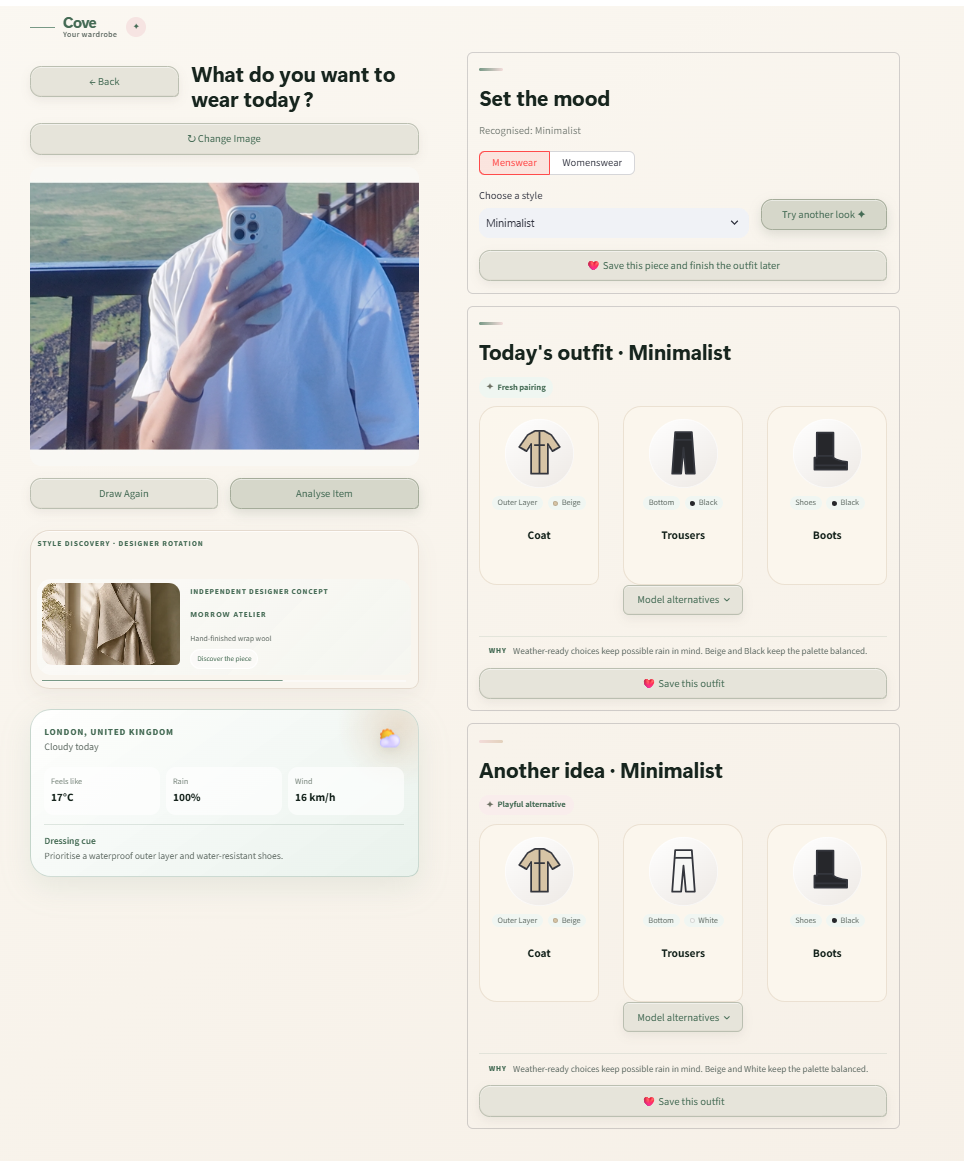
\includegraphics[width=0.82\textwidth]{assets/cove_recommendation.png}
  \caption{Cove recommendation interface showing the fixed garment, explicit
  clothing-range and style controls, abstract outfit alternatives and local
  save actions}
  \label{fig:cove-recommendation-interface}
\end{figure}

Table~\ref{tab:application-functions} records the responsibility of each core
application module. This division prevents the compatibility score from being
described as if it also performs recognition, weather validation or storage.

\begin{table}[htbp]
  \centering
  \caption{Core functions of the Cove prototype}
  \label{tab:application-functions}
  \small
  \begin{tabularx}{\textwidth}{@{}p{0.19\textwidth}p{0.25\textwidth}X@{}}
    \toprule
    \textbf{Module} & \textbf{Main input and output} & \textbf{Responsibility} \\
    \midrule
    Garment analysis & Selected crop $\rightarrow$ type, colour, style and embedding & Interprets the item supplied by the user and prepares its model representation. \\
    Candidate control & Context and fixed item $\rightarrow$ feasible states & Applies position, weather, style and clothing-range constraints. \\
    Compatibility ranking & Complete candidates $\rightarrow$ ordered scores & Scores relational coherence using the small project-specific head. \\
    Wardrobe management & Piece and outfit edits $\rightarrow$ local records and images & Saves, reuses, renames, groups and removes local wardrobe content. \\
    Fallback & Recognised item and context $\rightarrow$ rule-ranked outfit & Preserves basic operation when learned artefacts are absent or incompatible. \\
    \bottomrule
  \end{tabularx}
\end{table}

Persistent state is implemented through JSON documents and local image files,
while model and research outputs remain separate artefacts.
Figure~\ref{fig:local-data-relationships} presents these
logical relationships without implying tables, foreign keys or a database
engine that are not present in the implementation.

\begin{figure}[htbp]
  \centering
  \resizebox{\textwidth}{!}{%
  \begin{tikzpicture}[
    font=\small,
    entity/.style={draw=wmgdarkblue!60, rounded corners=2pt, align=left,
      minimum width=42mm, minimum height=19mm, fill=gray!6, inner sep=3mm},
    store/.style={entity, fill=wmgblue!10, draw=wmgblue!70},
    artefact/.style={entity, fill=green!6, draw=green!45!black},
    rel/.style={-{Latex[length=2mm]}, thick, draw=wmgdarkblue!65}
  ]
    \node[store] (wardrobe) {\textbf{wardrobe.json}\\version, pieces[], outfits[],\\outfit\_groups[]};
    \node[entity, below left=12mm and -2mm of wardrobe] (piece) {\textbf{Piece}\\id, position, type, colour,\\image\_path, source, created\_at};
    \node[entity, below right=12mm and -2mm of wardrobe] (outfit) {\textbf{Outfit}\\id, title, mood, style, group,\\four position values, created\_at};
    \node[entity, below=14mm of piece] (images) {\textbf{wardrobe\_images/}\\local PNG files referenced\\by Piece.image\_path};
    \node[entity, below=14mm of outfit] (prefs) {\textbf{user\_preferences.json}\\up to six saved cities};
    \node[store, right=20mm of outfit] (runtime) {\textbf{Application runtime}\\loads local user state and\\available model artefacts};
    \node[artefact, above=14mm of runtime] (model) {\textbf{Model artefacts}\\compatibility checkpoint and\\abstract prototype catalogue};
    \node[artefact, below=14mm of runtime] (results) {\textbf{Research outputs}\\evaluation JSON, manifests,\\hashes and training histories};

    \draw[rel] (wardrobe) -- node[left,font=\scriptsize]{contains} (piece);
    \draw[rel] (wardrobe) -- node[right,font=\scriptsize]{contains} (outfit);
    \draw[rel] (outfit) -- node[above,font=\scriptsize]{0--4 embedded piece values} (piece);
    \draw[rel] (piece) -- node[left,font=\scriptsize]{references} (images);
    \draw[rel] (wardrobe.east) -| (runtime.north west);
    \draw[rel] (prefs) -- node[below,font=\scriptsize]{read by} (runtime);
    \draw[rel] (model) -- node[right,font=\scriptsize]{loaded by} (runtime);
    \draw[rel,dashed] (model.east) -- ++(5mm,0) |- node[right,font=\scriptsize]{documented by} (results.east);
  \end{tikzpicture}}
  \caption{Logical relationships among local user data and model artefacts; the prototype uses files rather than a relational database}
  \label{fig:local-data-relationships}
\end{figure}


\begin{table}[htbp]
  \centering
  \caption{Local persistence and research artefacts}
  \label{tab:local-persistence}
  \small
  \begin{tabularx}{\textwidth}{@{}p{0.27\textwidth}p{0.27\textwidth}X@{}}
    \toprule
    \textbf{File or artefact} & \textbf{Principal contents} & \textbf{Role and relationship} \\
    \midrule
    \texttt{wardrobe.json} & Pieces, outfits and outfit groups & Local user store; each outfit contains values for the four supported positions. \\
    \texttt{wardrobe\_images/} & User garment PNG files & Image paths are referenced by saved piece records. \\
    \texttt{user\_preferences.json} & Saved cities & Read by the application to restore local location choices. \\
    Compatibility checkpoint & Model configuration, state and metadata & Reconstructs the selected compatibility scorer at runtime. \\
    Abstract prototype artefact & Candidate states and frozen embeddings & Supplies the product-independent candidate space for constrained search. \\
    Evaluation JSON and manifests & Metrics, histories, hashes and settings & Preserve the evidence chain; they are not user-profile records. \\
    \bottomrule
  \end{tabularx}
\end{table}

Supplementary software-design views are provided in
Appendix~\ref{app:software-design}. They include the implemented use cases,
overall component structure, recommendation-module dependencies, a logical
entity-relationship view and traceable user stories. The diagrams describe the
current prototype rather than an assumed enterprise architecture.

Result artefacts and checkpoints are larger than ordinary source files and may
not always be suitable for repository distribution. File hashes and documented
generation commands therefore provide an additional check that a locally held
artefact corresponds to the evaluated version. This approach does not replace
archival storage or full environment preservation, but it provides a practical
chain from processed data to training history, evaluation output and deployed
configuration.

\section{Research risks and mitigation}

The investigation involved data, methodological, ethical and operational
risks. These were considered during development rather than being listed only
after the experiments. The first concerned data provenance and permitted use.
The project therefore used documented secondary datasets and kept their roles
separate. Polyvore supplied compatibility labels, whereas Zara was limited to
recognition and feature-domain diagnostics. User photographs remained local
and were not incorporated into the research dataset. Any later public release would require a separate
check before third-party images or large derived artefacts could be
redistributed.

Dataset availability was not treated as blanket permission to redistribute
third-party content. The public-code package should exclude source dataset
images, item-level embeddings and catalogue artefacts. The compact learned-head
checkpoints contain model tensors, configuration and training metadata rather
than source images or product identifiers; their redistribution should still
be covered by a separate licence review before public release. This distinction
keeps the ethical approval boundary, research use and publication permission
from being treated as interchangeable.

A second risk was data leakage. Product overlap between training and test data
could allow a model to recognise garments seen during training instead of
learning relationships that transfer to unseen items. The published split was
used to reduce this risk, and candidate concepts were derived from the training
division rather than the test division. The local identifier audit confirmed
zero outfit-ID overlap but found the residual item-ID overlaps reported above,
so strict item-level separation cannot be claimed. Model selection and
temperature scaling used validation data, while the test set was reserved for
final evaluation. Repeatedly changing the model after inspecting test results
could still weaken test independence. The current test results are therefore
treated as final evidence for the selected model rather than as a further
tuning target.

The labels create a further interpretive risk. Positive examples are observed
Polyvore outfits, whereas negatives are constructed by replacing an item
within a broad category. A constructed negative is not proof that an outfit is
inherently unacceptable; it is a reproducible device for learning distinctions
within this dataset. Similarly, official FITB evaluation was restricted to
questions represented by the four supported positions and available
embeddings. Coverage is reported with accuracy so that performance on the
retained subset is not presented as a complete benchmark result. This follows
the principle that recommender metrics must be interpreted in relation to the
task and sampling protocol \parencite{herlocker2004evaluation}.

Overfitting and unstable model selection were addressed by recording training,
validation and test behaviour separately, using three random seeds for the
controlled architecture comparison and selecting checkpoints from validation
AUC. Confidence intervals were estimated for the principal test and paired
comparisons. Early stopping limits continued fitting after validation
performance stops improving, but does not remove a generalisation gap
\parencite{prechelt1998early}. The results therefore report both the close
validation--test result and the larger train--test difference.

Representation across clothing ranges was unequal. The retained FITB questions
and pure training examples were concentrated in womenswear, so the small
menswear subgroup could not support a reliable fairness comparison. The
interface asks users to choose a clothing range and does not infer gender from
an image. Menswear evidence is reported as sparse coverage rather than proof of
equal reliability. This does not resolve representational bias, but it avoids
automated gender classification and makes the evidential boundary explicit
\parencite{keyes2018misgendering,mehrabi2021bias}.

Finally, the deployed process could fail if model files, embeddings or
candidate records were unavailable, or if constraints removed every candidate
for a position. Release checks, deterministic seeds and recorded artefact paths
support reproducibility. Slot, weather and clothing-range constraints reject
infeasible combinations, while a deterministic rule-based fallback allows the
application to continue when learned artefacts cannot be loaded. These mitigations make failure conditions more
visible and bounded, without implying that technical testing removes all
social or external-validity risks.

\section{Summary}

The methodology combines a frozen visual encoder, a small project-specific
compatibility head and a constrained recommendation process. Controlled baselines, repeated
training runs, fill-in-the-blank evaluation, ablation experiments and system
tests were used to examine different aspects of performance. The following
chapter reports the corresponding results.
